% =============================================================================
% practica9.tex --- Chapter: Practice 9
% =============================================================================

\documentclass[../../__memoria.tex]{subfiles}

\begin{document}
\standalonecover
\pagestyle{cuerpo}

\graphicspath{{\subfix{../../Imagenes/}}{../../Imagenes/}{\subfix{img/}}{img/}}

\chapter[Práctica 9: Few-Shot Learning]{Cuaderno de Laboratorio --- Práctica 9: Aprendizaje con Pocos Ejemplos (Few-Shot Learning)}

En esta práctica exploramos el \textit{Few-Shot Learning} (aprendizaje con pocos ejemplos), una técnica útil cuando una clase nueva aparece después del entrenamiento y apenas tenemos muestras etiquetadas de ella. La idea clave es que, en lugar de reentrenar el modelo desde cero con los pocos datos disponibles, reutilizamos un modelo previamente entrenado como extractor de características. Sobre ese espacio de representación (embeddings), clasificamos las nuevas clases midiendo distancias a unos pocos prototipos calculados con los ejemplos disponibles.

El escenario que planteamos es el siguiente: entrenamos un clasificador CNN sobre el dataset MNIST, pero eliminando deliberadamente todas las imágenes del dígito 7 del entrenamiento. Después, convertimos ese clasificador en un extractor de características y comprobamos si podemos reconocer el dígito 7 usando solo 1 o 5 ejemplos. Así simulamos una situación real donde aparece una categoría que el modelo no ha visto antes.

% =============================================================================
\section[Tarea 1: Clasificador Base]{Tarea 1 --- El Mundo Sin Sietes}
% =============================================================================

\subsection{Carga y preprocesamiento}

Cargué el dataset MNIST y normalicé los píxeles al rango $[0, 1]$ dividiendo entre 255. Añadí una dimensión de canal para que las imágenes tuviesen forma $(28, 28, 1)$, que es la que espera una CNN. Después, eliminé del conjunto de entrenamiento todas las imágenes del dígito 7, quedándome con 53.735 muestras de las clases 0, 1, 2, 3, 4, 5, 6, 8 y 9. El conjunto de test se mantuvo completo con las 10.000 imágenes de los 10 dígitos.

\subsection{Arquitectura de la CNN}

Construí una red neuronal convolucional sencilla con la siguiente estructura:

\begin{itemize}
    \item \texttt{Conv2D(32, 3$\times$3, ReLU)} + \texttt{MaxPooling2D(2$\times$2)}
    \item \texttt{Conv2D(64, 3$\times$3, ReLU)} + \texttt{MaxPooling2D(2$\times$2)}
    \item \texttt{Flatten}
    \item \texttt{Dense(64, ReLU)} -- esta capa se llama \texttt{embedding} y es la que usaremos después
    \item \texttt{Dense(9, softmax)} -- clasificación sobre las 9 clases conocidas
\end{itemize}

Entrené el modelo con el optimizador Adam y pérdida \texttt{sparse\_categorical\_crossentropy} durante 3 épocas con lotes de 128 muestras.

\subsection{Análisis}

Eliminar el dígito 7 del entrenamiento no es un capricho: simula un escenario realista donde, después de haber entrenado un modelo, aparece una clase nueva que no estaba en los datos originales. Si el clasificador ha aprendido rasgos visuales generales (bordes, curvas, formas) en lugar de memorizar cada dígito, esos rasgos deberían ser útiles también para representar el 7. El experimento consiste precisamente en comprobar si eso es cierto.

% =============================================================================
\section[Tarea 2: Extractor]{Tarea 2 --- Extractor de Características}
% =============================================================================

\subsection{Construcción del extractor}

Una vez entrenado el clasificador, tomé el modelo y eliminé la última capa (la de clasificación \texttt{softmax}). El nuevo modelo recibe una imagen y devuelve la activación de la capa \texttt{embedding}, un vector de 64 componentes que describe la imagen en un espacio de características.

\subsection{Dimensión del embedding}

Al pasar una imagen de prueba por el extractor, el vector de salida tenía 64 dimensiones. Esto significa que cada imagen de 28$\times$28 = 784 píxeles se comprime a una representación de 64 números que capturan las características visuales más relevantes.

\subsection{Análisis}

Usar embeddings directamente es mucho mejor que comparar píxeles crudos por varias razones. La distancia entre píxeles de dos imágenes es muy sensible a cambios pequeños de posición, grosor o rotación; dos imágenes del mismo dígito pueden tener píxeles muy distintos si una está ligeramente desplazada. En cambio, los embeddings aprenden a ser invariantes a esas transformaciones: dos imágenes del mismo dígito, aunque estén escritas de forma distinta, deberían producir vectores cercanos en el espacio de 64 dimensiones.

% =============================================================================
\section[Tarea 3: Prototipos]{Tarea 3 --- Prototipos del Dígito 7}
% =============================================================================

\subsection{Construcción del support set}

Para cada enfoque, construí un \textit{support set} con los ejemplos de cada clase que se usan para definir los prototipos:
\begin{itemize}
    \item \textbf{1-shot}: 1 imagen del dígito 7 (extraída del test) más 1 imagen de cada clase conocida.
    \item \textbf{5-shot}: 5 imágenes del dígito 7 más 5 de cada clase conocida.
\end{itemize}

En total, para el enfoque 1-shot tenemos 10 prototipos (1 por clase), y para 5-shot también 10 prototipos, pero cada uno calculado a partir de 5 muestras.

\subsection{Cálculo del prototipo}

El prototipo de una clase es simplemente el vector medio de los embeddings de sus imágenes de apoyo:

\[
c_k = \frac{1}{|S_k|} \sum_{\mathbf{x}_i \in S_k} f(\mathbf{x}_i)
\]

donde $f(\mathbf{x}_i)$ es el embedding de la imagen $\mathbf{x}_i$ y $S_k$ es el support set de la clase $k$.

Es importante entender que un prototipo no es una imagen real: no podemos visualizarlo como un dibujo del dígito 7. Es un punto en el espacio de 64 dimensiones que representa la posición media de esa clase. Cuando tenemos más muestras (5-shot), ese punto medio es más estable y representativo que con una sola muestra (1-shot), que puede ser atípica.

\subsection{Prototipos multiclase}

Además del prototipo para el dígito 7, calculé prototipos para las clases conocidas usando el mismo procedimiento. Así, al clasificar una imagen de consulta, la comparamos contra los 10 prototipos (9 conocidos + 7) y la asignamos al más cercano.

% =============================================================================
\section[Tarea 4: Clasificación]{Tarea 4 --- Clasificación por Distancia}
% =============================================================================

\subsection{Métrica de distancia}

Para clasificar una imagen de consulta, calculé su embedding $f(\mathbf{q})$ y medí la distancia euclídea a cada prototipo:

\[
\hat{y} = \arg\min_k \| f(\mathbf{q}) - c_k \|_2
\]

La etiqueta asignada es la del prototipo más cercano. Implementé este cálculo usando la norma de NumPy con broadcasting para procesar todas las consultas a la vez.

\subsection{Conjunto de consulta (query set)}

Para la evaluación, construí un query set equilibrado con 100 imágenes de cada clase (100 $\times$ 10 = 1000 consultas en total), todas extraídas del conjunto de test. De esta forma, la métrica de accuracy refleja el rendimiento sobre las 10 clases con el mismo peso, sin importar el desbalanceo original de MNIST.

\subsection{Análisis}

La clasificación por distancia funciona bien cuando el espacio de embeddings separa correctamente las clases. Si el extractor ha aprendido representaciones útiles, las imágenes del mismo dígito deberían estar cerca entre sí y lejos de las de otros dígitos. En ese caso, el prototipo de cada clase cae cerca de su grupo y la distancia mínima asigna correctamente la mayoría de las consultas.

% =============================================================================
\section[Tarea 5: Comparativa]{Tarea 5 --- 1-Shot vs 5-Shot}
% =============================================================================

\subsection{Resultados}

\begin{table}[H]
    \centering
    \caption{Comparativa de accuracy entre 1-shot y 5-shot.}
    \label{tab:p9_comparativa}
    \begin{tabular}{lc}
        \toprule
        \textbf{Configuración} & \textbf{Accuracy sobre 1000 consultas} \\
        \midrule
        1-shot & 0.9120 \\
        5-shot & 0.9430 \\
        \bottomrule
    \end{tabular}
\end{table}

\begin{figure}[H]
    \centering
    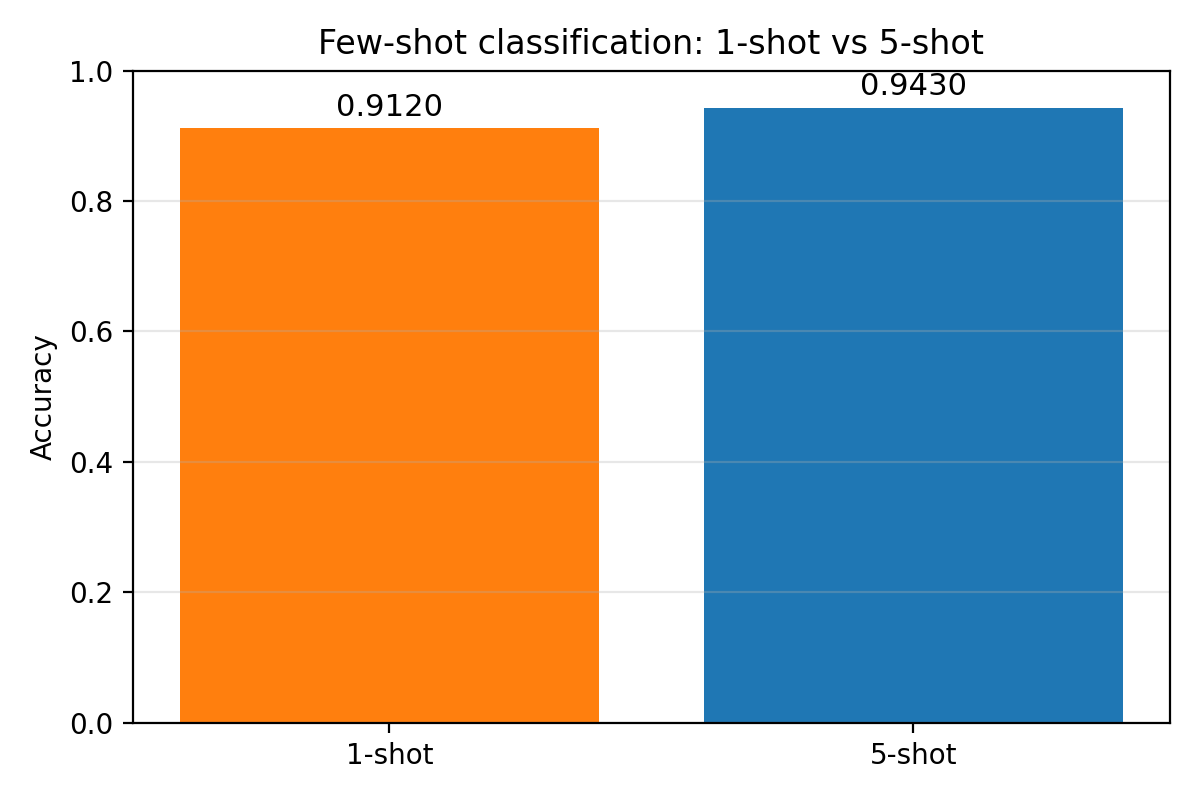
\includegraphics[width=0.65\linewidth]{img/fewshot_accuracy_comparison.png}
    \caption{Accuracy del clasificador por prototipos para 1-shot y 5-shot sobre el query set de 1000 imágenes.}
    \label{fig:p9_bars}
\end{figure}

\subsection{Análisis}

El enfoque 5-shot (94.30\,\%) supera al 1-shot (91.20\,\%) en 3.1 puntos porcentuales. La mejora era esperable: al promediar 5 ejemplares en lugar de 1, el prototipo es más robusto y menos sensible a que una de las imágenes de apoyo sea atípica (por ejemplo, un 7 mal escrito o con un trazo poco común). Con 1 solo ejemplo, si ese ejemplo no es representativo, el prototipo se desplaza y arrastra consigo los errores de clasificación de todas las consultas cercanas. Con 5 ejemplos, el promedio suaviza esas anomalías.

% =============================================================================
\section[Tarea 6: Visualización]{Tarea 6 --- Espacio de Características}
% =============================================================================

Para entender mejor cómo se organizan las clases en el espacio de embeddings, apliqué PCA a los vectores de 64 dimensiones para proyectarlos a 2 dimensiones y visualizarlos.

\begin{figure}[H]
    \centering
    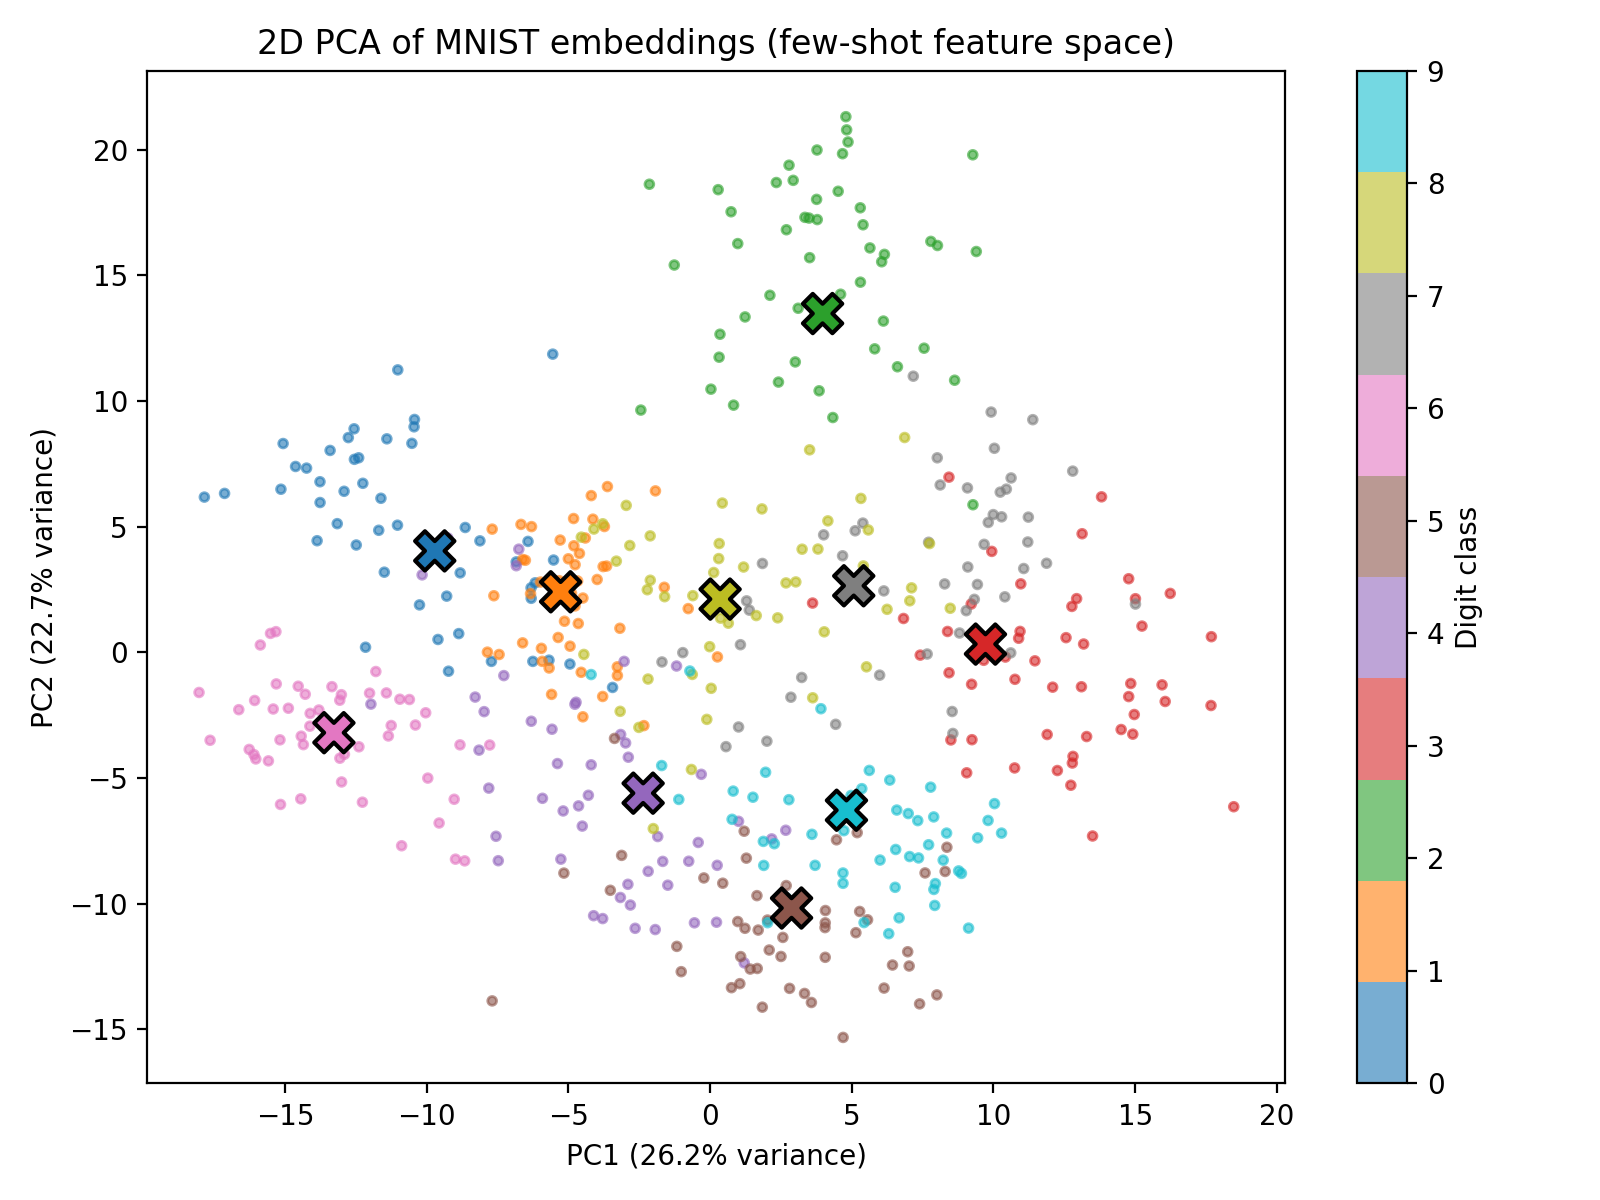
\includegraphics[width=0.78\linewidth]{img/fewshot_embeddings_pca.png}
    \caption{Proyección PCA de los embeddings de MNIST. Cada punto es una imagen del query set, coloreado según su clase real. Las marcas \texttt{X} negras muestran la posición de los prototipos (5-shot).}
    \label{fig:p9_pca}
\end{figure}

En la Figura~\ref{fig:p9_pca} se observa que la mayoría de los dígitos forman agrupaciones relativamente separadas. Los prototipos (marcados con \texttt{X}) caen dentro de sus respectivos grupos, lo que explica por qué la clasificación por distancia funciona. El dígito 7 aparece cerca del 9 y del 1, lo que tiene sentido visual: un 7 escrito a mano se parece a un 1 inclinado o a un 9 sin cerrar del todo. Esta proximidad es la principal fuente de errores de clasificación.

% =============================================================================
\section[Reto: Aplicación Real]{Reto --- Aplicación en un Problema Real}
% =============================================================================

\subsection{Ventajas del enfoque}

La principal ventaja de usar un extractor preentrenado es que no hay que entrenar un modelo desde cero cada vez que aparece una clase nueva. En una aplicación real (por ejemplo, detección de defectos en una fábrica donde pueden aparecer tipos de defecto no vistos antes), basta con calcular los prototipos de las nuevas clases con unos pocos ejemplos y ya se pueden clasificar. El coste computacional es mínimo comparado con reentrenar toda la red.

\subsection{Limitaciones críticas}

Sin embargo, el método tiene limitaciones importantes. La primera es la calidad del support set: si las pocas imágenes de apoyo no son representativas de la clase (por ejemplo, un 7 escrito de forma extraña), el prototipo se calcula mal y los errores se acumulan. La segunda es que el extractor puede no generar embeddings útiles para la clase nueva: si las características visuales de la clase nueva son muy distintas de las que vio durante el entrenamiento, el espacio de embeddings no las representará bien. Por último, clases visualmente similares (como el 7 y el 1, o el 3 y el 8) tienden a solaparse en el espacio de características, lo que provoca errores de clasificación difíciles de evitar incluso con más shots.

% =============================================================================
\section*{Conclusiones}
% =============================================================================

Esta práctica me sirvió para ver que un modelo entrenado para clasificar puede reutilizarse para algo muy distinto: generar representaciones. Lo que más me sorprendió es que, a pesar de haber eliminado completamente el dígito 7 del entrenamiento, el extractor era capaz de producir embeddings que diferenciaban el 7 de los demás dígitos con un 94.3\,\% de accuracy usando solo 5 ejemplos.

La diferencia entre 1-shot y 5-shot también fue interesante: 3 puntos de mejora pueden parecer poco, pero reflejan que el promedio de 5 muestras da un prototipo más estable. En un problema real donde cada error tenga un coste, merecería la pena etiquetar 5 ejemplos en lugar de 1.

El PCA de los embeddings confirmó visualmente que el espacio de características agrupa bien los dígitos similares, aunque también mostró solapamientos esperables (7 con 1 y 9). Si hiciese una siguiente iteración, probaría con un extractor más profundo (como una red preentrenada en ImageNet) o con métricas de distancia más sofisticadas. Pero para una primera toma de contacto con few-shot learning, los resultados me parecen muy buenos.

\end{document}
